\section{Introduction}
\label{sec:introduction}

GPU performance engineering is still fundamentally measurement-driven.
Developers usually optimize kernels by compiling candidate variants, running them on the target accelerator, profiling hardware counters, and then deciding whether to focus on computation, memory traffic, or both.
That workflow is already costly for humans, and it becomes even more expensive in agentic software-engineering loops where an LLM proposes many candidate edits and expects profiler feedback after each one \cite{liRiseAITeammates2025,gongLanguageModelsCode2025,ouyangKernelBenchCanLLMs2025,chenCUDALLMLLMsCan2025}.

\begin{figure}[t]
  \centering
  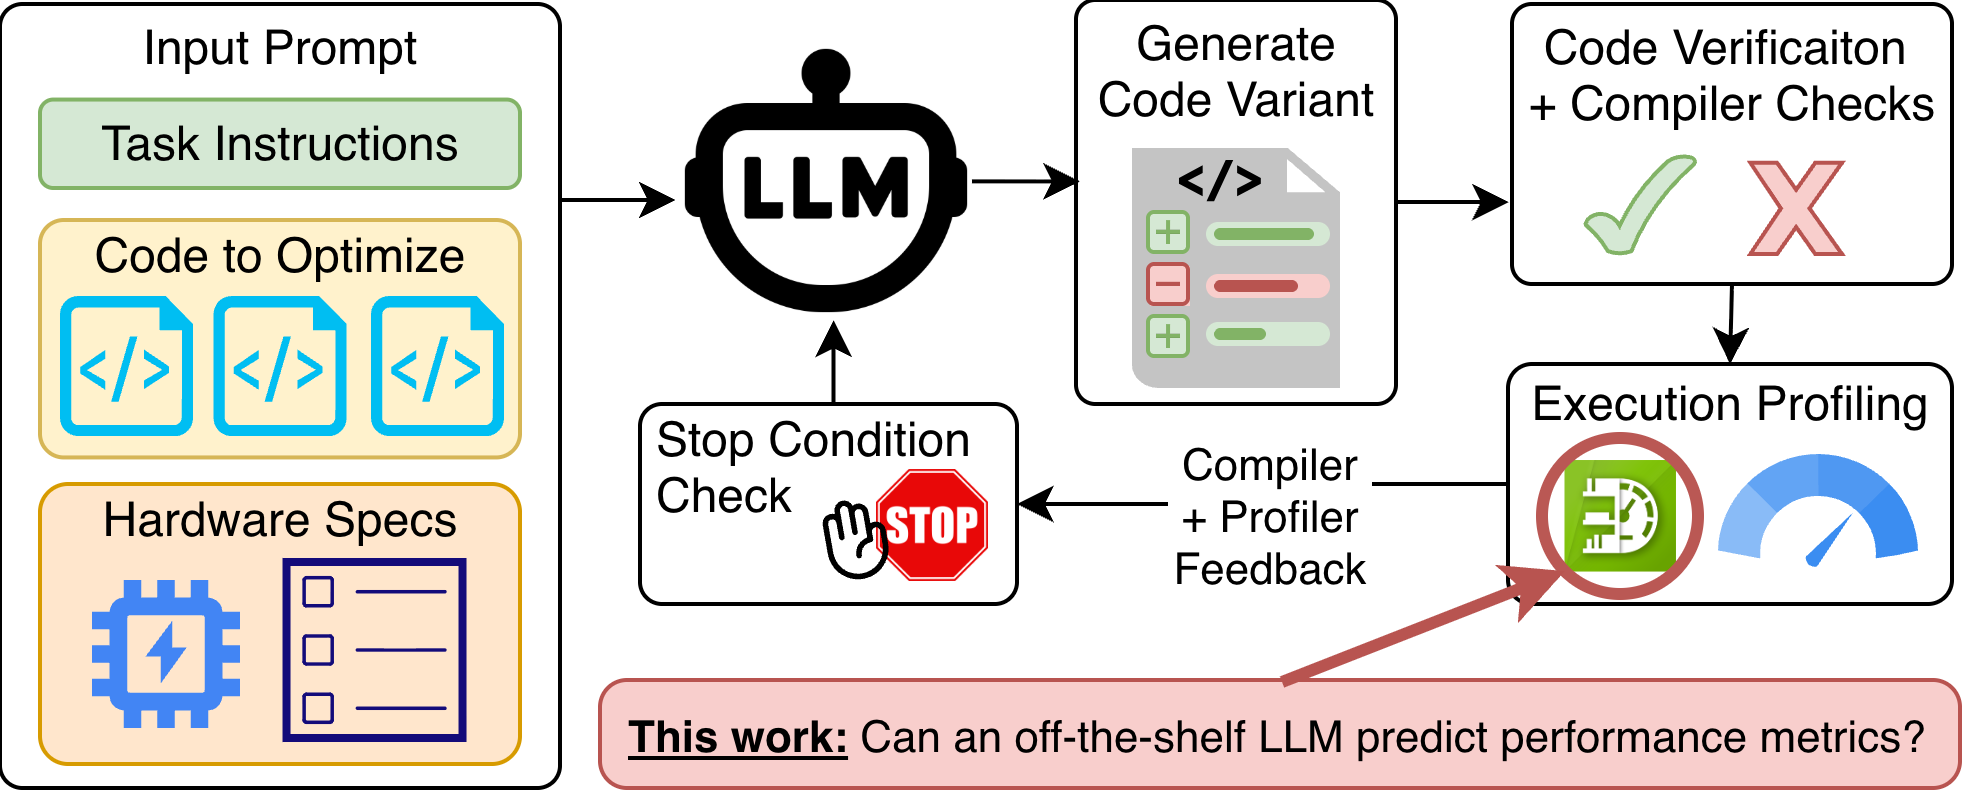
\includegraphics[width=\linewidth]{figures/optimization_loop.png}
  \caption{Profiler-in-the-loop GPU optimization is effective, but it assumes repeated access to the target accelerator.
  We study whether off-the-shelf LLMs can classify a kernel's bandwidth-bound versus compute-bound Roofline regime earlier in that loop, from software artifacts alone, before runtime profiling is available.}
  \Description{A diagram contrasting the usual compile-run-profile optimization loop with an earlier execution-free triage step that classifies a kernel's Roofline regime from software artifacts before scarce GPU profiling time is used.}
  \label{fig:optimization-loop}
\end{figure}

In practice, target-GPU access is often the bottleneck.
Accelerators may be rationed on a shared cluster, unavailable in early development, blocked by missing system dependencies, or simply too expensive to occupy for speculative triage.
The practical question is therefore not ``can an LLM replace a profiler?'' but a narrower one that a developer or coding agent faces \emph{before} a profiling run is available: on a given target GPU, is this kernel likely to be limited by data movement or by computation?

That bandwidth-bound versus compute-bound (\bandwidthbound/\computebound) decision is the first branch of Roofline analysis \cite{samuelwilliamsRooflineInsightfulVisual2009}, and it is the one that determines which optimization direction is even worth attempting.
It is also fundamentally a \emph{classification}, not a precise number: a developer who learns that a kernel is firmly compute-bound can act on that without knowing its arithmetic intensity to two decimals.
We therefore make Roofline-regime classification the primary object of study, and treat the underlying Roofline Arithmetic Intensity (\rai) as a diagnostic that explains \emph{why} a classification is right or wrong rather than as the headline deliverable.

We study three off-the-shelf LLMs in two evidence settings.
The \sourceonly setting provides only pre-compilation artifacts---source files, build commands, runtime arguments, and GPU specifications---and corresponds to early development, code review, or agent planning.
The \sourcesass setting adds the target kernel's SASS disassembly.
Crucially, SASS is obtained by \emph{cross-compilation} (for example, \texttt{nvcc -arch=sm\_90} followed by \texttt{cuobjdump -sass}) and therefore requires no target hardware; both settings are execution-free at prediction time.
Comparing them isolates what compiler lowering adds over source-visible semantics.

We organize the study around three research questions:
\begin{itemize}[leftmargin=1.2em]
  \item \textbf{RQ1.} Can off-the-shelf LLMs classify a kernel's \bandwidthbound/\computebound Roofline regime from source artifacts alone, and for which precisions?
  \item \textbf{RQ2.} What does cross-compiled SASS add to that classification, and why?
  \item \textbf{RQ3.} How do the resulting signals compare---in accuracy and in cost---against lightweight static baselines and against profiling itself?
\end{itemize}

To answer them we build on 95 HeCBench CUDA and OpenMP programs.
They expose 254 first-invocation GPU kernels and 1{,}016 profiled samples across an RTX~3080, A10, A100, and H100.
For each sample the models predict launch dimensions, per-precision FP16/FP32/FP64 floating-point work, and DRAM bytes read and written; we derive both \rai and its \bandwidthbound/\computebound side relative to each GPU's Roofline balance point.
For fair cross-model comparison we use the 732 samples completed by all three models in both evidence settings.

Three findings matter most.

First (RQ1), source artifacts already support good single-precision regime classification but are blind to half precision.
\opus classifies the \sourceonly FP32 regime at 0.940 nonzero balanced accuracy (and FP64 at 0.755), and even the budget \gptoss reaches 0.875 for FP32.
For FP16, however, all three models sit at the 0.500 chance baseline from source alone.

Second (RQ2), the FP16 gap is an evidence gap, not a model-capability gap, and it closes with compilation.
The decisive half-precision arithmetic is compiler-synthesized---packed \texttt{HFMA2} operations that are not syntactically present in source---so source-only reasoning cannot see it.
Adding cross-compiled SASS lifts FP16 \bandwidthbound/\computebound balanced accuracy from 0.500 to 0.984 for \opus and 0.870 for \gptfivefour.
This is the paper's clearest result: \emph{compilation, not execution, is what half-precision Roofline reasoning requires}, and compilation is available without the target GPU.

Third (RQ3), these signals are cheap relative to profiling, and they form a tier.
A \sourceonly FP32 regime classification from the budget model costs on the order of \$0.0006 per kernel---orders of magnitude below occupying a target GPU for a profiling run---while the frontier+SASS configuration is a premium tier that additionally resolves FP16.
Lightweight deterministic and learned static baselines recover part of the same signal and even win in a few regimes (notably \sourcesass FP64), so the deployable shape is a cost-tiered cascade among execution-free strategies rather than an LLM-only oracle.
Numeric \rai estimation is accurate only in identifiable regimes and is best used as a diagnostic and a coarse profiling-priority hint, not as a runtime substitute.

Our contribution is squarely about software engineering.
We study how execution-relevant software artifacts can support AI-assisted performance reasoning before execution.

More concretely, we make four contributions:
\begin{itemize}[leftmargin=1.2em]
  \item We formulate execution-free Roofline-regime classification as a software-engineering task for early GPU-kernel triage, with software artifacts as inputs and profiler-derived \bandwidthbound/\computebound labels as ground truth.
  \item We show that the source-versus-compilation evidence boundary, not model choice, governs half-precision triage, and give the mechanistic compiler-synthesized-FP16 explanation.
  \item We quantify the accuracy/cost tiering of off-the-shelf prompting against context-only, deterministic, and lightweight learned static baselines, and against the cost of profiling.
  \item We package the benchmark---source, build context, runtime arguments, SASS, profiler-derived labels, and model outputs---as a reusable artifact for execution-free GPU performance reasoning, documenting limits that future work can address with repeated-query and reasoning-versus-memorization studies.
\end{itemize}

The remainder is organized as follows.
Section~\ref{sec:related-work} positions our work relative to Roofline analysis, execution-free GPU performance prediction, and LLM-based optimization.
Sections~\ref{sec:task-methodology} and \ref{sec:study-design} define the prediction task and study design.
Section~\ref{sec:results} answers the research questions.
Sections~\ref{sec:discussion} and \ref{sec:threats} translate the findings into implications and limitations for ICSE readers, and Section~\ref{sec:conclusion} concludes.
